\documentclass{standalone}
\usepackage{tikz}
\usetikzlibrary{patterns, positioning}
\usetikzlibrary{shapes.misc}
\usepackage[outline]{contour}
\contourlength{1.5pt} 
\usepackage[sfdefault]{ClearSans} %% option 'sfdefault' activates Clear Sans as the default text font
\usepackage[T1]{fontenc}

\begin{document}
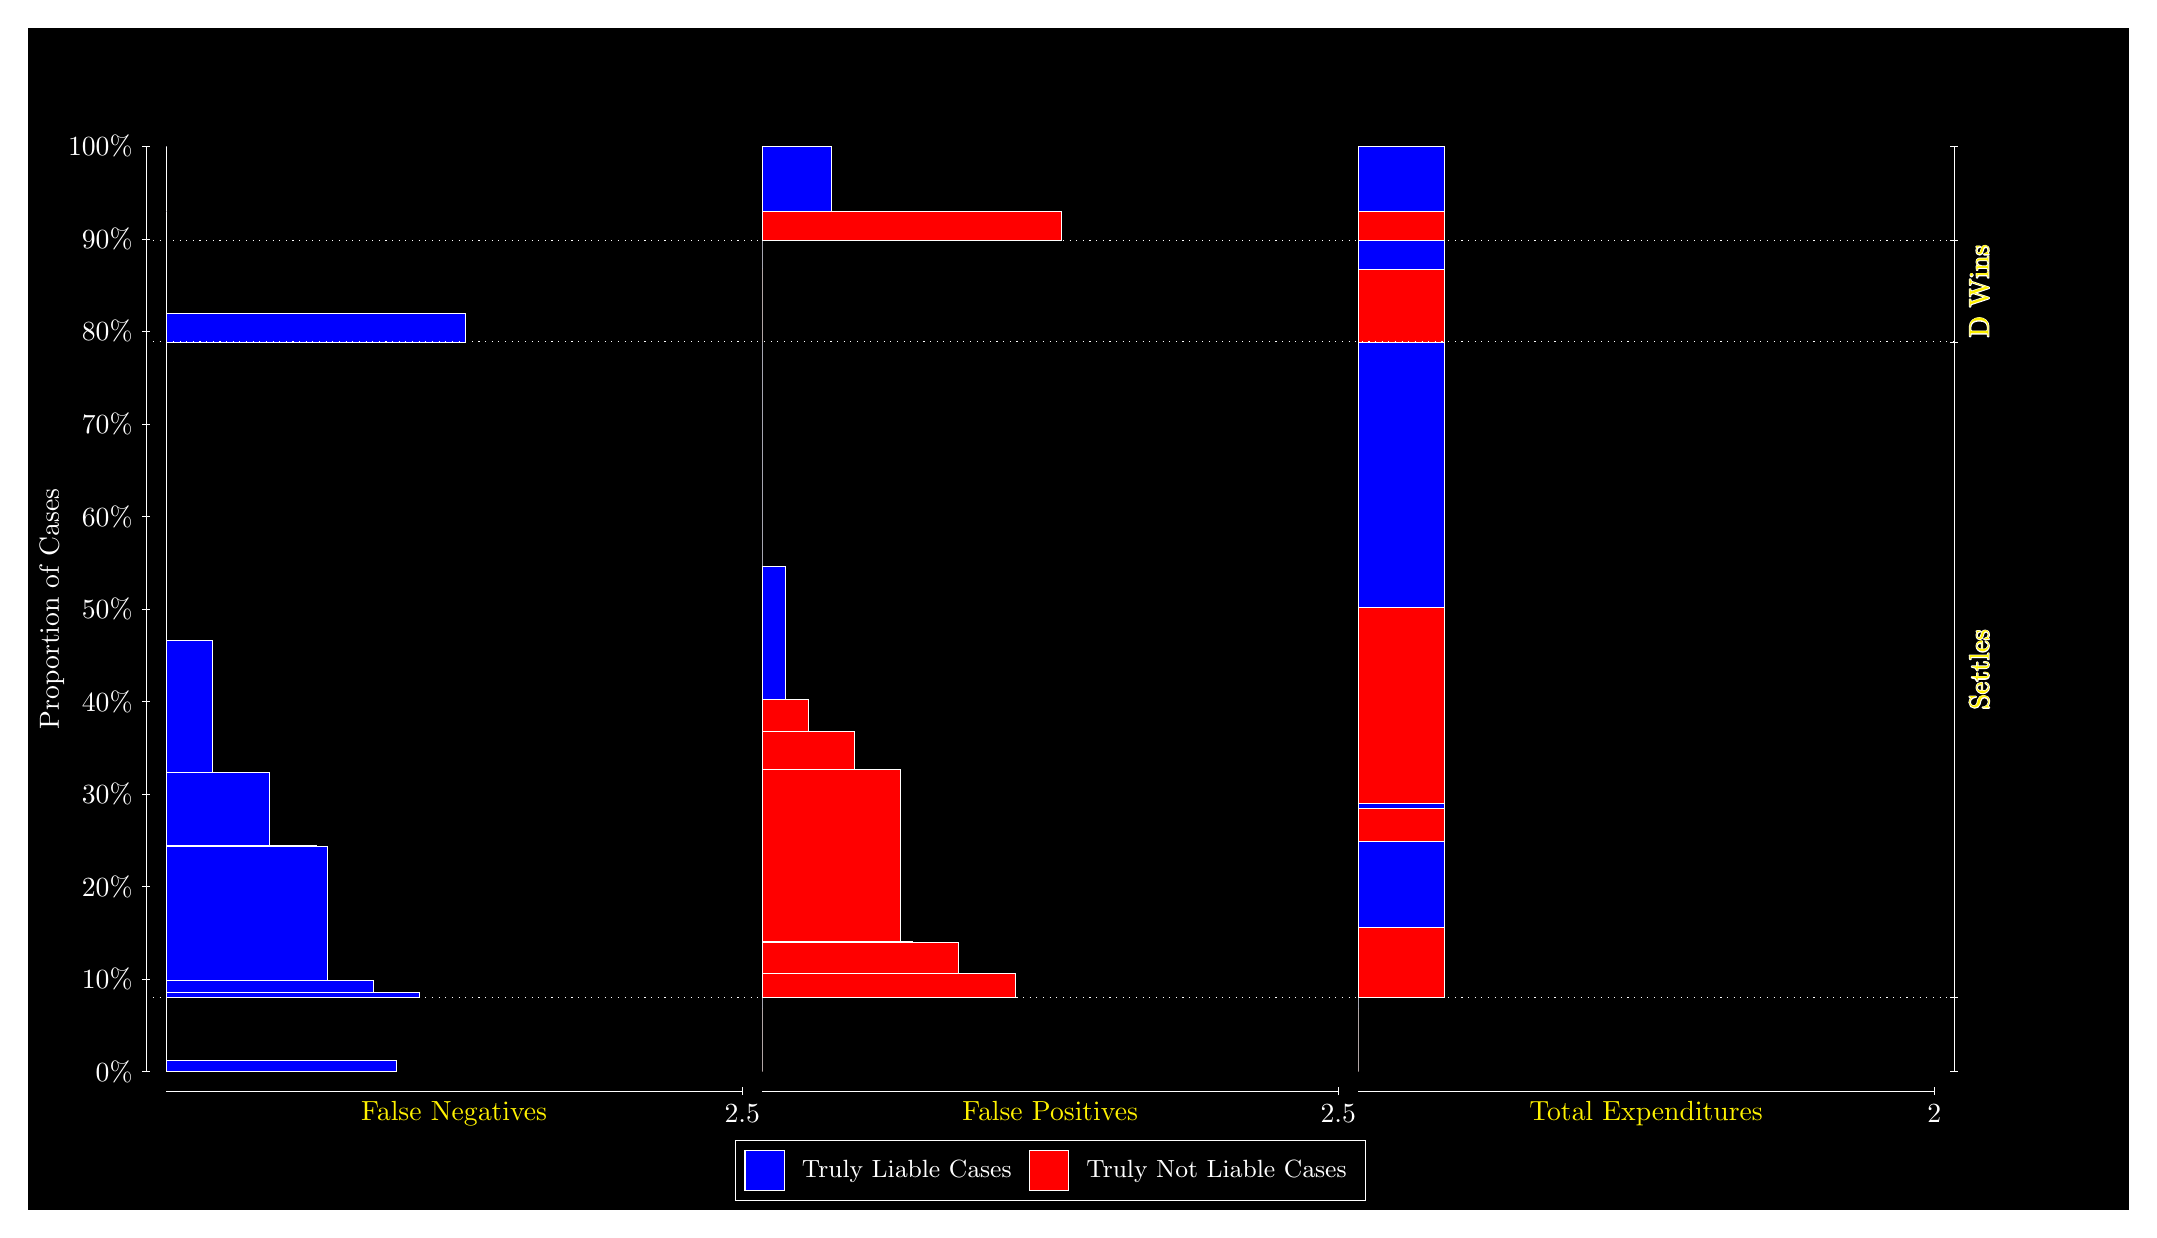
\begin{tikzpicture}
\draw[fill=black] (0,0) rectangle (26.667,15);
\draw[white, very thin] (1.5,1.75) -- (1.5,13.5);
\node[rotate=90, text=white, anchor=center] at (0.3, 7.625) {Proportion of Cases};
\draw[white, very thin] (1.45,1.75) -- (1.55,1.75);
\node[text=white, anchor=east] at (1.45, 1.75) {0\%};
\draw[white, very thin] (1.45,2.925) -- (1.55,2.925);
\node[text=white, anchor=east] at (1.45, 2.925) {10\%};
\draw[white, very thin] (1.45,4.1) -- (1.55,4.1);
\node[text=white, anchor=east] at (1.45, 4.1) {20\%};
\draw[white, very thin] (1.45,5.275) -- (1.55,5.275);
\node[text=white, anchor=east] at (1.45, 5.275) {30\%};
\draw[white, very thin] (1.45,6.45) -- (1.55,6.45);
\node[text=white, anchor=east] at (1.45, 6.45) {40\%};
\draw[white, very thin] (1.45,7.625) -- (1.55,7.625);
\node[text=white, anchor=east] at (1.45, 7.625) {50\%};
\draw[white, very thin] (1.45,8.8) -- (1.55,8.8);
\node[text=white, anchor=east] at (1.45, 8.8) {60\%};
\draw[white, very thin] (1.45,9.975) -- (1.55,9.975);
\node[text=white, anchor=east] at (1.45, 9.975) {70\%};
\draw[white, very thin] (1.45,11.15) -- (1.55,11.15);
\node[text=white, anchor=east] at (1.45, 11.15) {80\%};
\draw[white, very thin] (1.45,12.325) -- (1.55,12.325);
\node[text=white, anchor=east] at (1.45, 12.325) {90\%};
\draw[white, very thin] (1.45,13.5) -- (1.55,13.5);
\node[text=white, anchor=east] at (1.45, 13.5) {100\%};

\draw[white, very thin] (24.457,1.75) -- (24.457,13.5);
\draw[white, very thin] (24.407,1.75) -- (24.507,1.75);
\node[anchor=west] at (24.407, 1.75) {};
\draw[white, very thin] (24.407,2.6953) -- (24.507,2.6953);
\node[anchor=west] at (24.407, 2.6953) {};
\draw[white, very thin] (24.407,11.017) -- (24.507,11.017);
\node[anchor=west] at (24.407, 11.017) {};
\draw[white, very thin] (24.407,12.305) -- (24.507,12.305);
\node[anchor=west] at (24.407, 12.305) {};
\draw[white, very thin] (24.407,13.5) -- (24.507,13.5);
\node[anchor=west] at (24.407, 13.5) {};

\draw[white, very thin, fill=blue] (1.75,1.75) rectangle (4.6775,1.8987);
\draw[white, very thin, fill=red] (1.75,1.8987) rectangle (1.75,2.6953);
\draw[white, very thin, fill=blue] (1.75,2.6953) rectangle (4.9703,2.7598);
\draw[white, very thin, fill=blue] (1.75,2.7598) rectangle (4.3848,2.9138);
\draw[white, very thin, fill=blue] (1.75,2.9138) rectangle (3.7993,4.612);
\draw[white, very thin, fill=blue] (1.75,4.612) rectangle (3.6529,4.6273);
\draw[white, very thin, fill=blue] (1.75,4.6273) rectangle (3.0674,5.5507);
\draw[white, very thin, fill=blue] (1.75,5.5507) rectangle (2.3355,7.2303);
\draw[white, very thin, fill=red] (1.75,7.2303) rectangle (1.75,11.017);
\draw[white, very thin, fill=blue] (1.75,11.017) rectangle (5.5558,11.379);
\draw[white, very thin, fill=red] (1.75,11.379) rectangle (1.75,12.305);
\draw[white, very thin, fill=red] (1.75,12.305) rectangle (1.75,12.671);
\draw[white, very thin, fill=blue] (1.75,12.671) rectangle (1.75,13.5);
\draw[white, very thin, fill=red] (9.3189,1.75) rectangle (9.3189,2.5466);
\draw[white, very thin, fill=blue] (9.3189,2.5466) rectangle (9.3189,2.6953);
\draw[white, very thin, fill=red] (9.3189,2.6953) rectangle (12.539,3.0007);
\draw[white, very thin, fill=red] (9.3189,3.0007) rectangle (11.807,3.3858);
\draw[white, very thin, fill=red] (9.3189,3.3858) rectangle (11.222,3.4031);
\draw[white, very thin, fill=red] (9.3189,3.4031) rectangle (11.075,5.5859);
\draw[white, very thin, fill=red] (9.3189,5.5859) rectangle (10.49,6.074);
\draw[white, very thin, fill=red] (9.3189,6.074) rectangle (9.9044,6.4824);
\draw[white, very thin, fill=blue] (9.3189,6.4824) rectangle (9.6116,8.162);
\draw[white, very thin, fill=blue] (9.3189,8.162) rectangle (9.3189,11.017);
\draw[white, very thin, fill=red] (9.3189,11.017) rectangle (9.3189,11.943);
\draw[white, very thin, fill=blue] (9.3189,11.943) rectangle (9.3189,12.305);
\draw[white, very thin, fill=red] (9.3189,12.305) rectangle (13.125,12.671);
\draw[white, very thin, fill=blue] (9.3189,12.671) rectangle (10.197,13.5);
\draw[white, very thin, fill=red] (16.888,1.75) rectangle (16.888,2.5466);
\draw[white, very thin, fill=blue] (16.888,2.5466) rectangle (16.888,2.6953);
\draw[white, very thin, fill=red] (16.888,2.6953) rectangle (17.986,3.5858);
\draw[white, very thin, fill=blue] (16.888,3.5858) rectangle (17.986,4.6786);
\draw[white, very thin, fill=red] (16.888,4.6786) rectangle (17.986,5.087);
\draw[white, very thin, fill=blue] (16.888,5.087) rectangle (17.986,5.1515);
\draw[white, very thin, fill=red] (16.888,5.1515) rectangle (17.986,7.6397);
\draw[white, very thin, fill=blue] (16.888,7.6397) rectangle (17.986,11.017);
\draw[white, very thin, fill=red] (16.888,11.017) rectangle (17.986,11.943);
\draw[white, very thin, fill=blue] (16.888,11.943) rectangle (17.986,12.305);
\draw[white, very thin, fill=red] (16.888,12.305) rectangle (17.986,12.671);
\draw[white, very thin, fill=blue] (16.888,12.671) rectangle (17.986,13.5);
\draw[white, dotted] (1.5,2.6953) -- (24.457,2.6953);
\draw[white, dotted] (1.5,11.017) -- (24.457,11.017);
\draw[white, dotted] (1.5,12.305) -- (24.457,12.305);
\draw[white, very thin] (1.75,1.5) -- (9.0689,1.5);
\node[text=yellow, anchor=north] at (5.4094, 1.5) {False Negatives};
\draw[white, very thin] (9.0689,1.45) -- (9.0689,1.55);
\node[text=white, anchor=north] at (9.0689, 1.45) {2.5};

\draw[white, very thin] (9.3189,1.5) -- (16.638,1.5);
\node[text=yellow, anchor=north] at (12.978, 1.5) {False Positives};
\draw[white, very thin] (16.638,1.45) -- (16.638,1.55);
\node[text=white, anchor=north] at (16.638, 1.45) {2.5};

\draw[white, very thin] (16.888,1.5) -- (24.207,1.5);
\node[text=yellow, anchor=north] at (20.547, 1.5) {Total Expenditures};
\draw[white, very thin] (24.207,1.45) -- (24.207,1.55);
\node[text=white, anchor=north] at (24.207, 1.45) {2};


\node[text=yellow, centered, rotate=90] at (24.777, 6.8564) {\contour{white}{Settles}};
\node[text=yellow, centered, rotate=90] at (24.777, 11.661) {\contour{white}{D Wins}};


\draw (12.978300999999998,1.5) node[draw=none] (baseCoordinate) {};
\begin{scope}[align=center]
        \matrix[scale=0.5, draw=white, below=0.5cm of baseCoordinate, nodes={draw}, column sep=0.1cm]{
            \node[rectangle, draw, minimum width=0.5cm, minimum height=0.5cm, fill=blue] {}; &
            \node[draw=none, font=\small, text=white] (B) {Truly Liable Cases}; &
            \node[rectangle, draw, minimum width=0.5cm, minimum height=0.5cm, fill=red] {}; &
            \node[draw=none, font=\small, text=white] (B) {Truly Not Liable Cases}; \\
            };
\end{scope}

\end{tikzpicture}
\end{document}